Nas seções anteriores foram coletados alguns indícios para seleção do descritores combinadas com a melhor técnica de normalização, menor número de características. Por isso, para consolidar os dados anteriores e evitar superestimação dos resultados encontrados foi utilizado a técnica de validação cruzada estratificada em 10 partições.

\subsubsection{Descritor LBP}
Com relação a acurácia as médias e devio padrão foram respectivamente: LR: 69\%, 16\%; KNN: 46\%, 24\%; SVM: 64\%, 22\%; MLP: 71\%, 18\%. Estes dados podem ser vistos na Tabela ~\ref{tab:result_lbp} e Figura~\ref{fig:box_result_lbp}.


\begin{table}[!htbp]
	\caption{Acurácia dos classificadores utilizando o descritor LBP}
	\begin{center}
		\begin{tabular}{|c|c|c|}
			\hline
			& Média & Desvio Padrão \\
			\hline
			MLP       & 71\% & 18\% \\
			LR        & 69\% & 16\% \\
			SVM       & 64\% & 22\% \\
			KNN       & 46\% & 24\% \\
			\hline
		\end{tabular}
		\label{tab:result_lbp}
	\end{center}
\end{table}

\begin{figure}[!htbp]
	\centering
	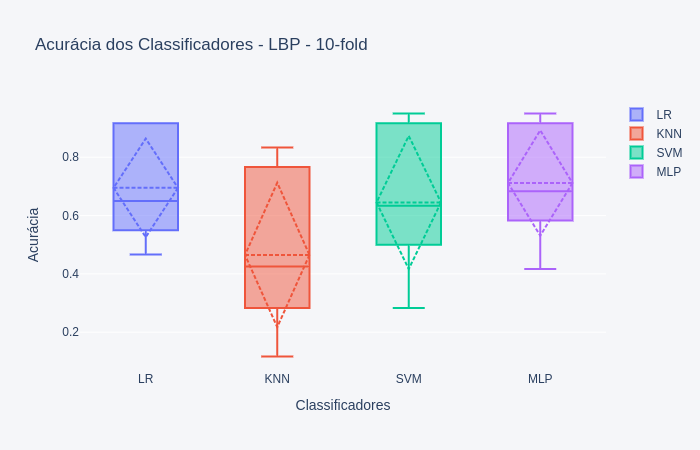
\includegraphics[width=1.0\linewidth,clip=true,trim=0cm 0cm 0cm 0cm, keepaspectratio=true]{box_result_lbp.png}
	\caption{Média e Desvio Padrão da Acurácia com o descritor LBP}
	\label{fig:box_result_lbp}
\end{figure}

\subsubsection{Descritor Gabor}
Com o descritor Gabor a média e desvio padrão foram respectivamente: LR: 28\%, 26\%; KNN: 25\%, 13\%; SVM: 29\%, 30\%; MLP: 27\%, 28\%.. Estes dados podem ser vistos na Tabela ~\ref{tab:result_gabor} e Figura~\ref{fig:box_result_gabor}. 


\begin{table}[!htbp]
	\caption{Acurácia dos classificadores utilizando o descritor Gabor}
	\begin{center}
		\begin{tabular}{|c|c|c|}
			\hline
			& Média & Desvio Padrão \\
			\hline
			SVM       & 29\% & 30\% \\
			LR        & 28\% & 26\% \\
			MLP       & 27\% & 28\% \\
			KNN       & 25\% & 13\% \\
			\hline
		\end{tabular}
		\label{tab:result_gabor}
	\end{center}
\end{table}

\begin{figure}[!htbp]
	\centering
	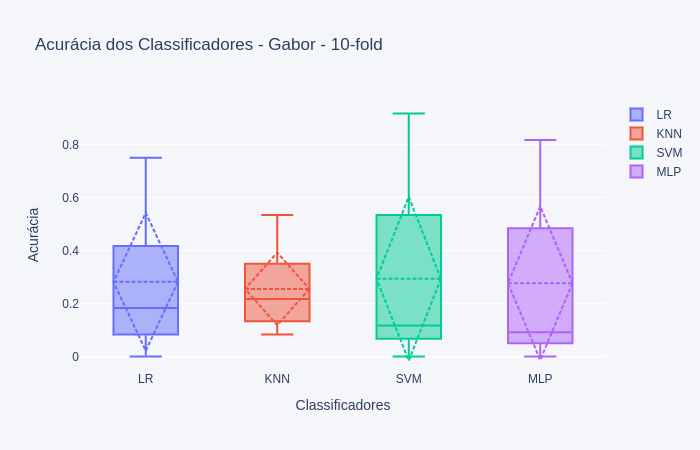
\includegraphics[width=1.0\linewidth,clip=true,trim=0cm 0cm 0cm 0cm, keepaspectratio=true]{box_result_gabor.png}
	\caption{Média e Desvio Padrão da Acurácia com o descritor Gabor}
	\label{fig:box_result_gabor}
\end{figure}